\part{Telas}

\section{Tela de Abertura}

\begin{enumerate}

\item Lista das opções para o jogador \\\\
O jogador terá na tela inicial as opções de iniciar o jogo e vizualizar a tela de créditos. \\

\item Interface com a tela \\\\
Todas as telas terão alguma relação sistema-usuário, algumas por meio do teclado e outras por meio do mouse. \\

\item Modo de salvar e/ou carregar um arquivo de progresso \\\\
No jogo não terá um modo de salvar progresso consequentemente não haverá também a modo de carregar um arquivo de progresso pois o jogo é muito curto não havendo a necessidade dessas funcionalidades, então caso o jogador queira sair no meio da fase, ele perderá todo seu progresso até o momento. \\

\item Músicas \\\\
Serão implementados no jogo três músicas, uma tocará no menu, uma na corrida e a última na tela de game over.

Na questão do gráfico, não se sabe ainda qual será o nível gráfico do jogo então ainda não é possível ter noção se o usuário terá a opção de aumentar ou diminuir essa característica. \\

\end{enumerate}

\label{1}
\begin{figure}[!h]
	\centering
		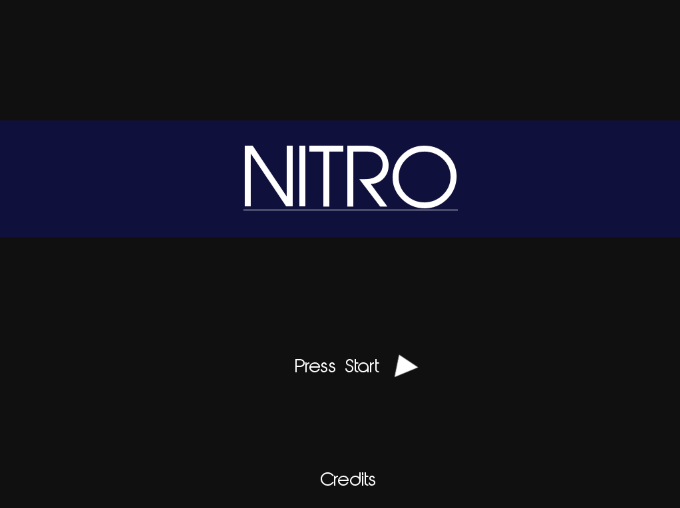
\includegraphics[scale=0.3]{figuras/tela_inicial}
	\caption{Imagem da tela inicial}
\end{figure}

\section{Outras telas}

\subsection{Tela de Créditos}

A tela de créditos aparecerá quando o jogador conseguir ganhar o jogo e se a opção no menu inicial for selecionada, nela passarão os nomes dos desenvolvedores, da materia e da universidade. \\\\\\\\\\

\begin{figure}[!h]
	\centering
		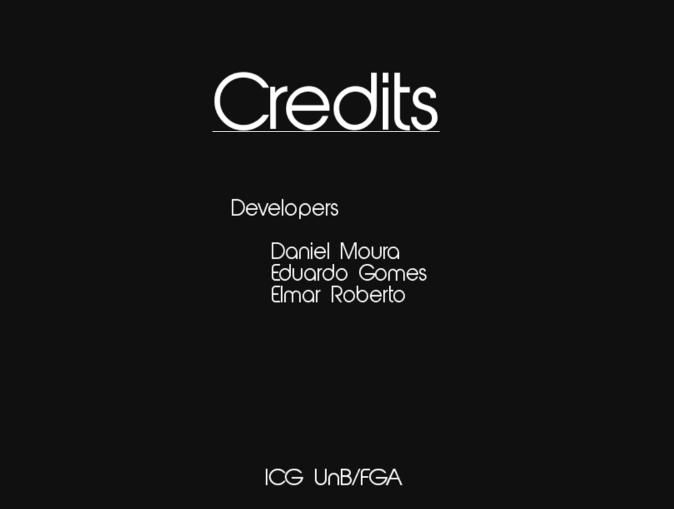
\includegraphics[scale=0.3]{figuras/creditos}
	\caption{Imagem da tela de créditos}
\end{figure}

\subsection{Tela de Game Over}

A tela de game over irá aparecer caso acabe a gasolina ou o carro saia da pista. \\

\begin{figure}[!h]
	\centering
		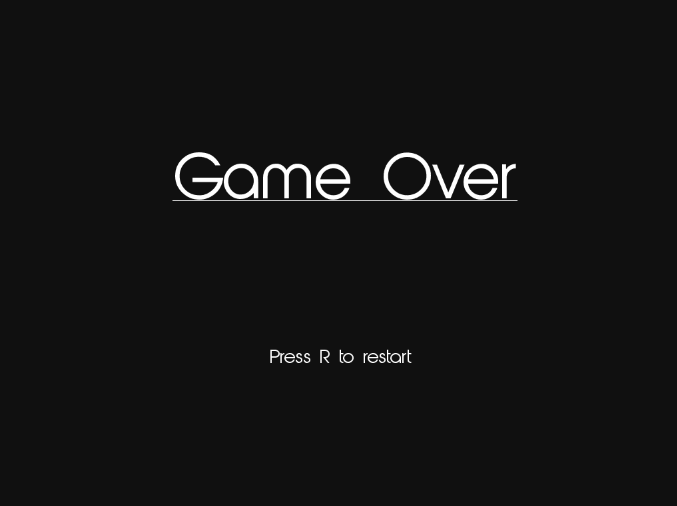
\includegraphics[scale=0.3]{figuras/game_over}
	\caption{Imagem da tela de Game Over}
\end{figure}

\subsection{Tela de Jogo}

\begin{figure}[!h]
	\centering
		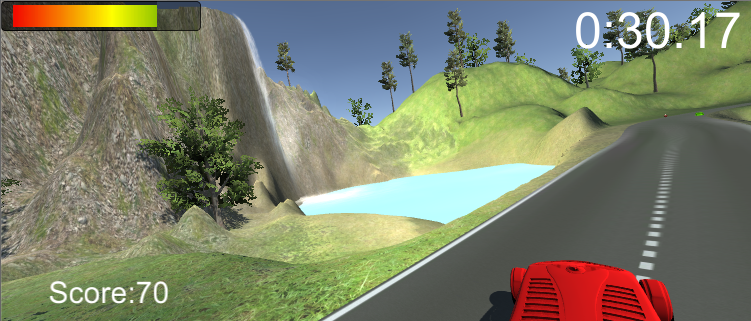
\includegraphics[scale=0.4]{figuras/tela_jogo}
	\caption{Imagem da tela de Jogo}
\end{figure}